%% Thesis template for The Hong Kong Polytechnic University %%
%% Author: Bailun JIANG %%
%% Date:   March 2023 %%

\documentclass[12pt]{book}

%% Packages %%
\usepackage[a4paper, inner=3cm, outer=2cm, height = 9in]{geometry} % Margin settings
\usepackage{setspace}           % Line spacing
\usepackage[pdftex]{graphicx}   % Inserting images
\usepackage{cite}               % Citations
\usepackage{afterpage}          % Blank pages
\usepackage[T1]{fontenc}        % Font settings 
\usepackage{titlesec}           % Title spacings
\usepackage{fancyhdr}           % Header&footer settings
\usepackage{acronym}            % For acronym. To use without list of abbreviations: \usepackage[nolist]{acronym}
\usepackage{subcaption}         % For subcaption
\usepackage{siunitx}            % For units
\usepackage[cmex10]{amsmath}    % For equations
\usepackage{amssymb}            % For bold
\usepackage{url}
\PassOptionsToPackage{hyphens}{url}\usepackage{hyperref}
\usepackage{multirow} 

\usepackage{etoolbox}
\preto\section\acresetall

\setlength{\parskip}{0pt}       % No extra space between paragraphs
\allowdisplaybreaks             % Allow display(e.g., equation) break

%% General Settings %%
\onehalfspacing                 % Line spacing
\graphicspath{{figures/}}       % Image settings
\DeclareGraphicsExtensions{.pdf,.jpeg,.png}
\fontfamily{qtm}\selectfont     % Font selection
\titlespacing*{\section}        % Title spacings
{0pt}{5.5ex plus 1ex minus .2ex}{4.3ex plus .2ex}
\titlespacing*{\subsection}
{0pt}{5.5ex plus 1ex minus .2ex}{4.3ex plus .2ex}

%% Header & Footer Settings %%
\fancypagestyle{plain}{         % Page style used for first page of chapter
\fancyhf{}                      % Clear existing header&footer entries
\fancyfoot[LE,RO]{\thepage} 
\renewcommand{\headrulewidth}{0pt}
\renewcommand{\footrulewidth}{0pt}}
\pagestyle{fancy}               % For general pages
\fancyhf{}
\setlength{\headheight}{14.5pt}
\fancyfoot[LE,RO]{\thepage}     % Page number position
\renewcommand{\headrulewidth}{0pt}

%% Document %%
\begin{document}

    \pagenumbering{gobble}
    \newcommand{\thesistitle}{Thesis Title}
\newcommand{\authorname}{Author Name}
\newcommand{\authorinfo}{Author Info}
\newcommand{\thesisdescription}{A thesis submitted in partial fulfilment of the requirements of the degree of Master of Philosophy/Doctor of Philosophy}
\newcommand{\deptname}{Department Name}
\newcommand{\univname}{The Hong Kong Polytechnic University}
\newcommand{\supervisorname}{Title FirstName LastName}
\newcommand{\yearofaward}{YYYY/YYYY}
\newcommand{\submissiondate}{MM/YYYY}

%% Functions

\newcommand\printlogo{
    
\includegraphics[keepaspectratio=true, width=0.4\pdfpagewidth]{images/template/polyu_logo.png}
}

\newcommand\blankpage{
    \null
    \newpage}

%% Cover Page

\printlogo
\begin{center}

\vspace*{.1\textheight}
{\LARGE \textbf{\MakeUppercase{\thesistitle}}\par}\vspace{0.5cm}

\vspace*{.05\textheight}
{\LARGE \textbf{\MakeUppercase{\authorname}}\par}\vspace{0.5cm}

\vspace*{.05\textheight}
{\LARGE \textbf{\authorinfo}\par}\vspace{0.5cm}

\vspace*{.25\textheight}
{\LARGE \textbf{\univname}\par}\vspace{0.5cm}

\vspace*{.05\textheight}
{\LARGE \textbf{\MakeUppercase{\yearofaward}}\par}\vspace{0.5cm}

\vfill
\end{center}
\afterpage{\blankpage}

%% Title Page

\printlogo
\begin{center}

\vspace*{.1\textheight}
{\LARGE \univname \par}\vspace{0.5cm}

\vspace*{.05\textheight}
{\LARGE \deptname \par}\vspace{0.5cm}

\vspace*{.05\textheight}
{\LARGE \textbf{\thesistitle}\par}\vspace{0.5cm}

\vspace*{.05\textheight}
{\large \authorname \par}\vspace{0.5cm}

\vspace*{.2\textheight}
{\large \thesisdescription \par}\vspace{0.5cm}

\vspace*{.05\textheight}
{\large \submissiondate \par}\vspace{0.5cm}

\vfill
\end{center}
\afterpage{\blankpage}
    \newpage
    \pagenumbering{Roman}

    \chapter*{\MakeUppercase{Certificate of Originality}}
\addcontentsline{toc}{chapter}{Certificate of Originality}
\label{chap::certificateoforiginality}

I hereby declare that this thesis is my own work and that, to the best of my knowledge and belief, it reproduces no material previously published or written, nor material that has been accepted for the award of any other degree or diploma, except where due acknowledgement has been made in the text.

\vspace{1cm}
\hfill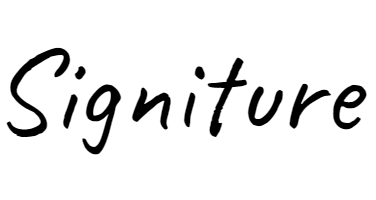
\includegraphics[keepaspectratio=true, width=0.15\pdfpagewidth]{images/template/signature.png}

{\large \hfill \authorname \par}\vspace{0.5cm}
    \chapter*{Abstract}
\addcontentsline{toc}{chapter}{Abstract}
\label{chap::abstract}
This is the abstract of your thesis.

\noindent \textbf{Keywords}: first-kw; second-kw; third-kw

\newpage
    \chapter*{Acknowledgements}
\addcontentsline{toc}{chapter}{Acknowledgements}
\label{chap::acknowledgements}

Write your acknowledgements.

    \tableofcontents
    \addcontentsline{toc}{chapter}{Contents}
    
    \listoffigures
    \addcontentsline{toc}{chapter}{List of Figures}
    \label{chap::listoffigures}
    
    \listoftables
    \addcontentsline{toc}{chapter}{List of Tables}
    \label{chap::listoftables}

    \chapter*{List of Abbreviations}
\addcontentsline{toc}{chapter}{List of Abbreviations}
\label{chap::listofabbreviations}

\begin{acronym}     % Define your acronyms below
    \acro{ML}{Machine Learning}
\end{acronym}

\afterpage{\null \newpage}
\newpage
    \newpage

    \renewcommand{\headrulewidth}{0.5pt}
    \fancyhead[LE,RO]{\nouppercase{\leftmark}}
    \pagenumbering{arabic}
    
    \chapter{Introduction}
\label{chap::introduction}

Write the introduction of your document.

This is an example of a footnote \footnote{Example of a footnote}:

This is an example of \textbf{boldface} text.

This is an example of \textit{italicized} text.

This is an example of a bullet-list:
\begin{itemize}
    \item First item
    \item Second item
\end{itemize}

This is an example of an ordered list:
\begin{enumerate}
    \item First element
    \item Second element
\end{enumerate}

This is an example of a reference to a different section of the document: Section~\ref{chap::literature_review}.

\noindent You can avoid indentation by using the \textbackslash noindent command

\section{Subsection of the Introduction}
\label{subsec::subsectionoftheintroduction}
If you want, you can add more depth to your document by using \textit{subsections}.

\subsection{Subsubsection of the Subsection of the Introduction}
\label{subsubsec::subsubsectionofthesubsectionoftheintroduction}
You can also use a subsubsection.
    \chapter{Literature Review}
\label{chap::literature_review}

This is the section describing the related work and outlining the research gap that your document is addressing.

This is an example of an ``in-text'' citation: \cite{jordan2015machine}.

Remember to insert each entry to the \textit{references.bib} file.

\textbf{Do not} describe concepts that have limited connection to your goal. Whoever is going to read this thesis is meant to be an ``expert''!

Use schemas or figures if necessary: they help a lot in understanding. If you take the schemas from previous work, do cite them in the caption. Figures can be cited with \textbackslash ref command such as Figure \ref{fig::example_picture}.

\begin{figure}[!htbp]
    \centering
    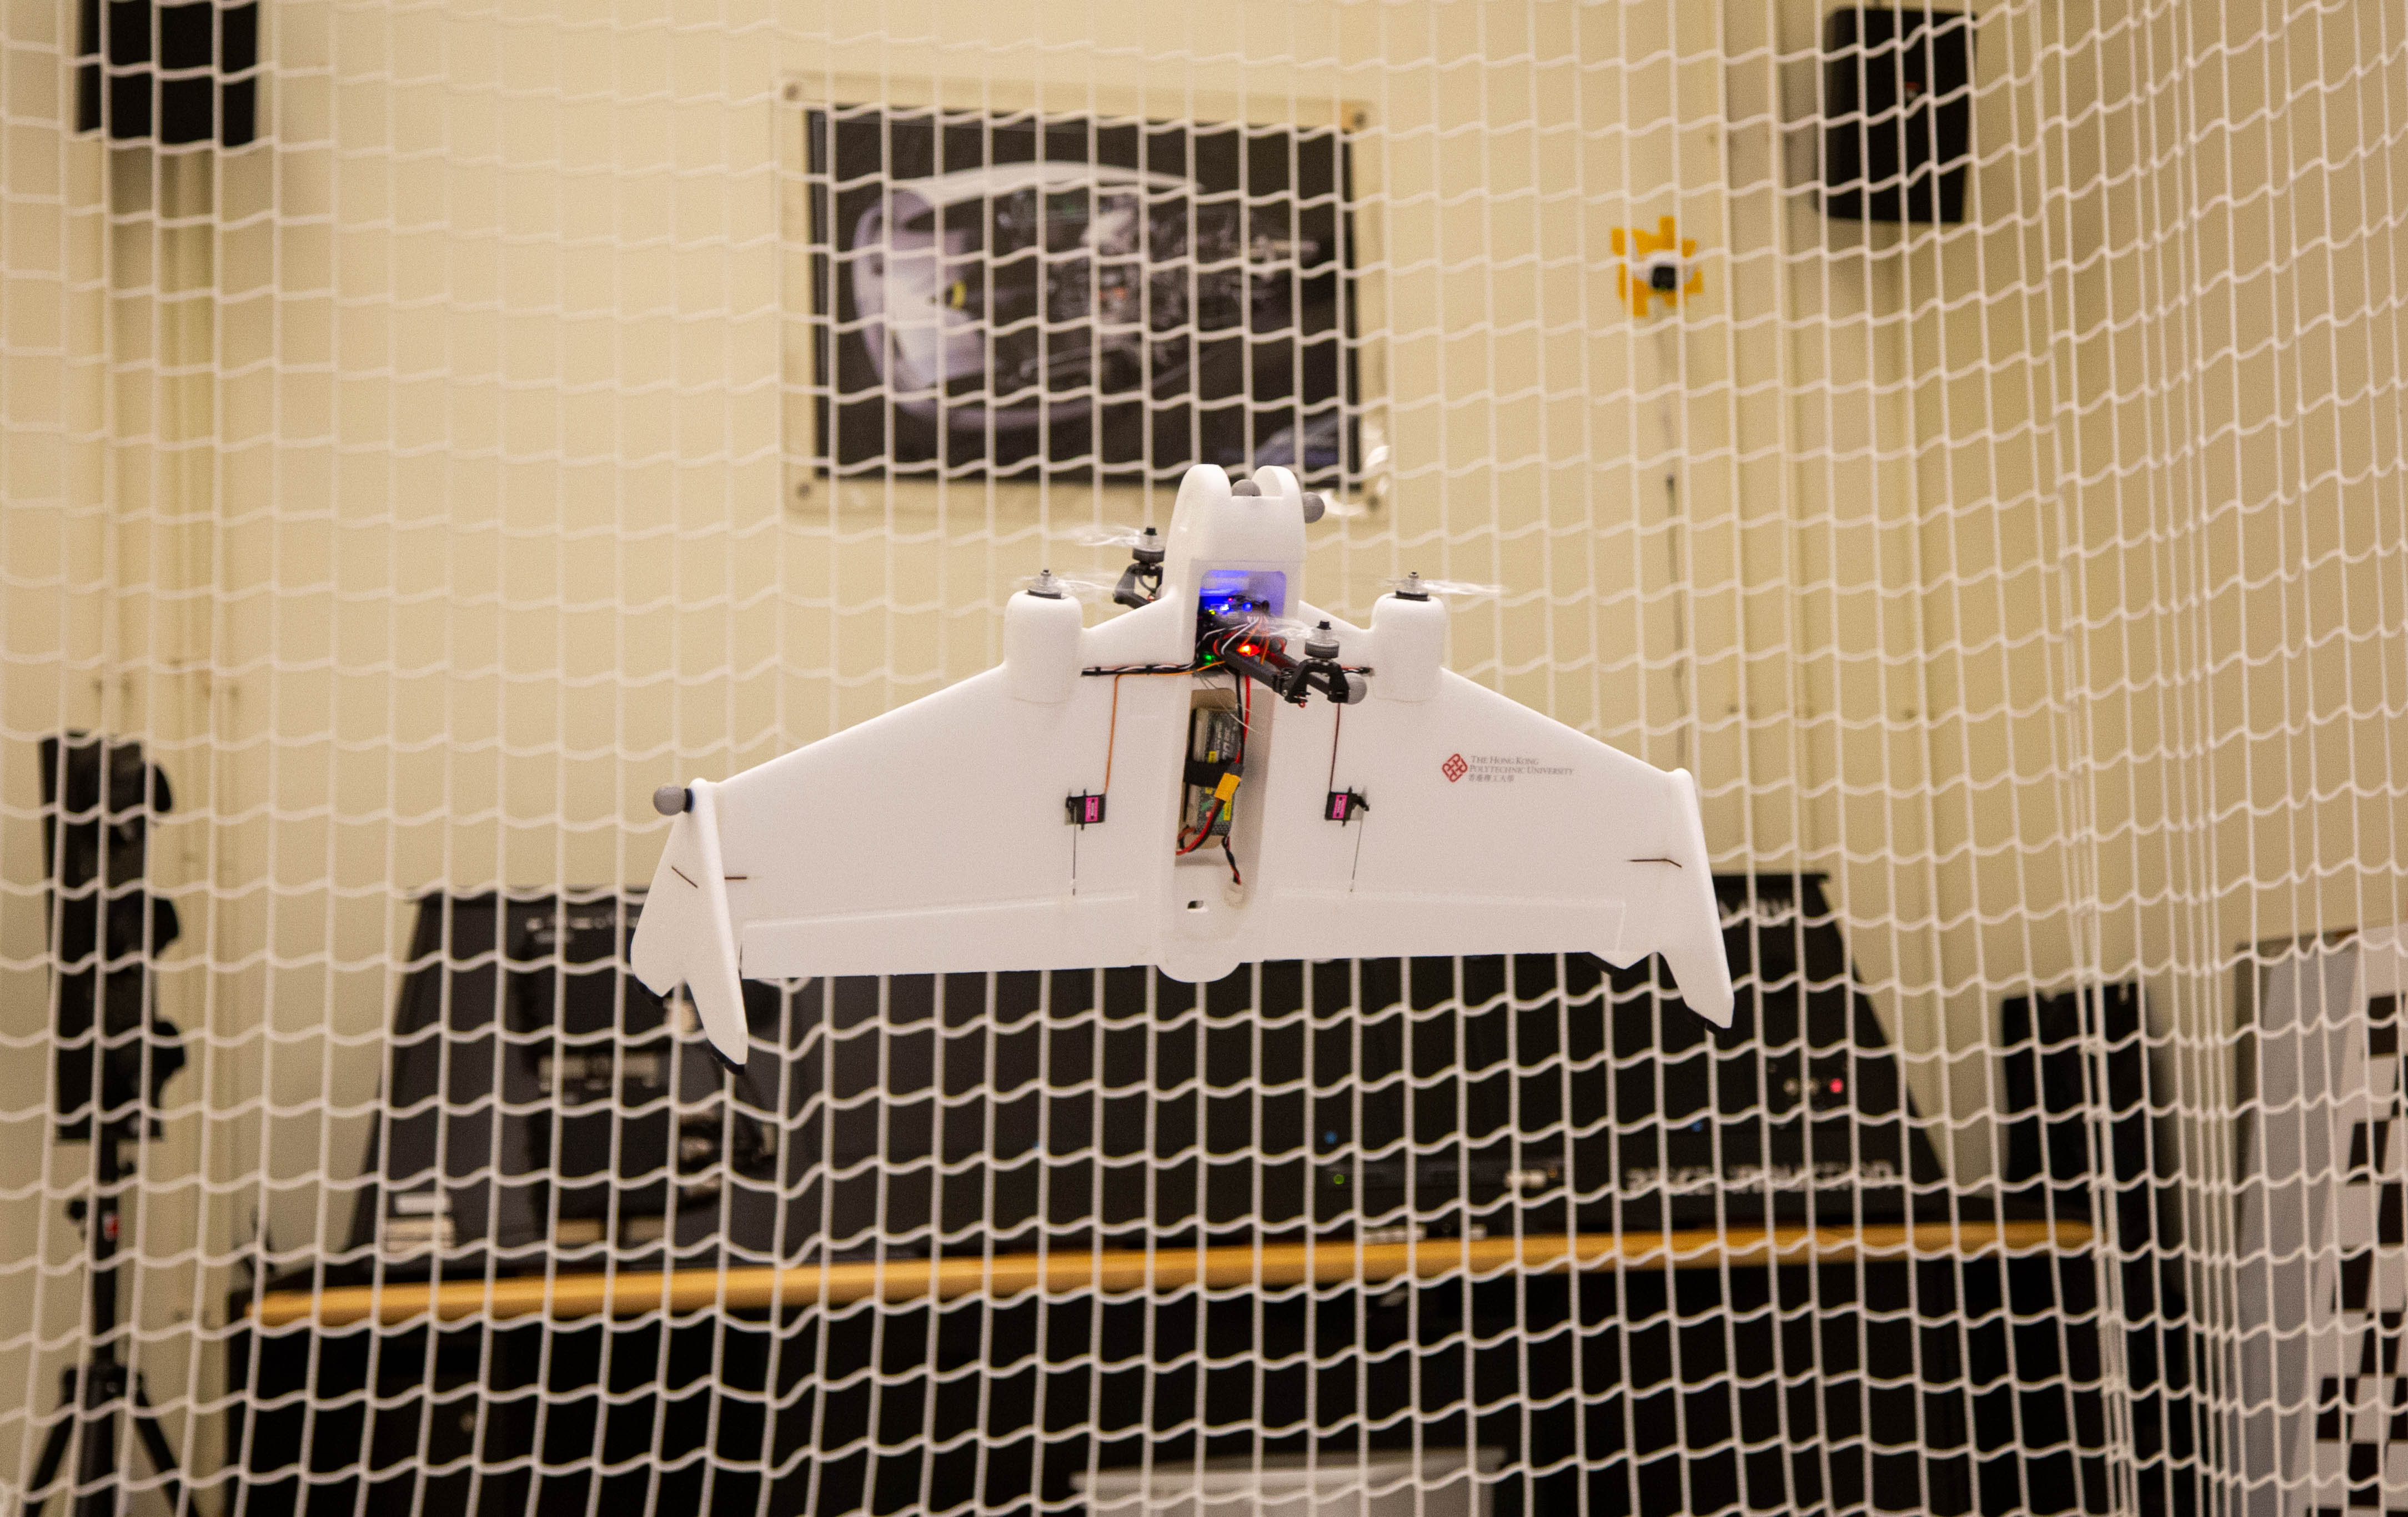
\includegraphics[width=0.75\columnwidth]{images/figures/example_figure.jpg}
    \caption{The caption of figures goes BELOW the figure.}
    \label{fig::example_picture}
\end{figure}

All acronyms should be defined in \textit{acronym.tex} and referred to with \textbackslash ac command. The first referred acronym will display the whole name such as \ac{ML}, and only abbreviations will be displayed afterwards such as \ac{ML}.
    \chapter{Methodology}
\label{chap::methodology}
This chapter presents a thorough description of the methods used for data collection in this thesis.

\section{Overview}
\label{sec::overview}
The aim of this thesis is to ...

\begin{table}[!htbp]
    \centering
    \caption{The caption of tables goes ABOVE the table}
    \begin{tabular}{c|c}
         row 1 column 1 & row 1 column 2  \\
         row 2 column 1 & row 2 column 2 
    \end{tabular}
    
    \label{tab::table_template}
\end{table}

We can see from Table~\ref{tab::table_template} that...
    \chapter{Results and Discussion}
\label{chap::resultsanddiscussion}

(this is a free section, depending on your thesis, it can have a different title and a different structure / goal than the one provided in this template)

\section{Implementation}
\label{sec::implementation}

(this is a free section, depending on your thesis, it can have a different title and a different structure / goal than the one provided in this template)
\section{Results}
\label{sec::results}

(this is a free section, depending on your thesis, it can have a different title and a different structure / goal than the one provided in this template)
\section{Discussion}
\label{sec::discussion}

(this is a free section, depending on your thesis, it can have a different title and a different structure / goal than the one provided in this template)
    \chapter{Conclusions and Future Work}
\label{chap::conclusionsandfuturework}

(The conclusions are always at the end of the thesis.)

Summarize what has been done in thesis, and how the findings can be helpful for future research, and also discuss some potential avenues of future work.

    \cleardoublepage
    \phantomsection
    \addcontentsline{toc}{chapter}{Bibliography}
    \bibliographystyle{IEEEtran}
    \bibliography{references}
    
\end{document}
